\section{Comparing conditional acceptance and the Gibbs sampling method.}

The Metropolis-Hastings sampling algorithm uses a conditional acceptance ratio. The Gibbs sampling method, which is what we have mostly used throughout this thesis, removes this condition and accepts every proposed sample state. With Gibbs sampling we can vectorize the process, resulting in a substantial decrease in computation time. Here we would like to see if the acceptance criteria, based on the RBM's internal energy, can improve prediction accuracy by giving a better approximation of the machine state. 

\def \mgeps {-2}
\def \mgW {0.1}
\def \mgC {70000}

For comparison we will use the Lipkin model with $16$ particles and $\varepsilon = \mgeps$ and $W = \mgW$, checking the accuracy of the two sampling methods for $V = -1 \rightarrow V = 0$. 

\begin{figure}[H]
  \begin{center}
    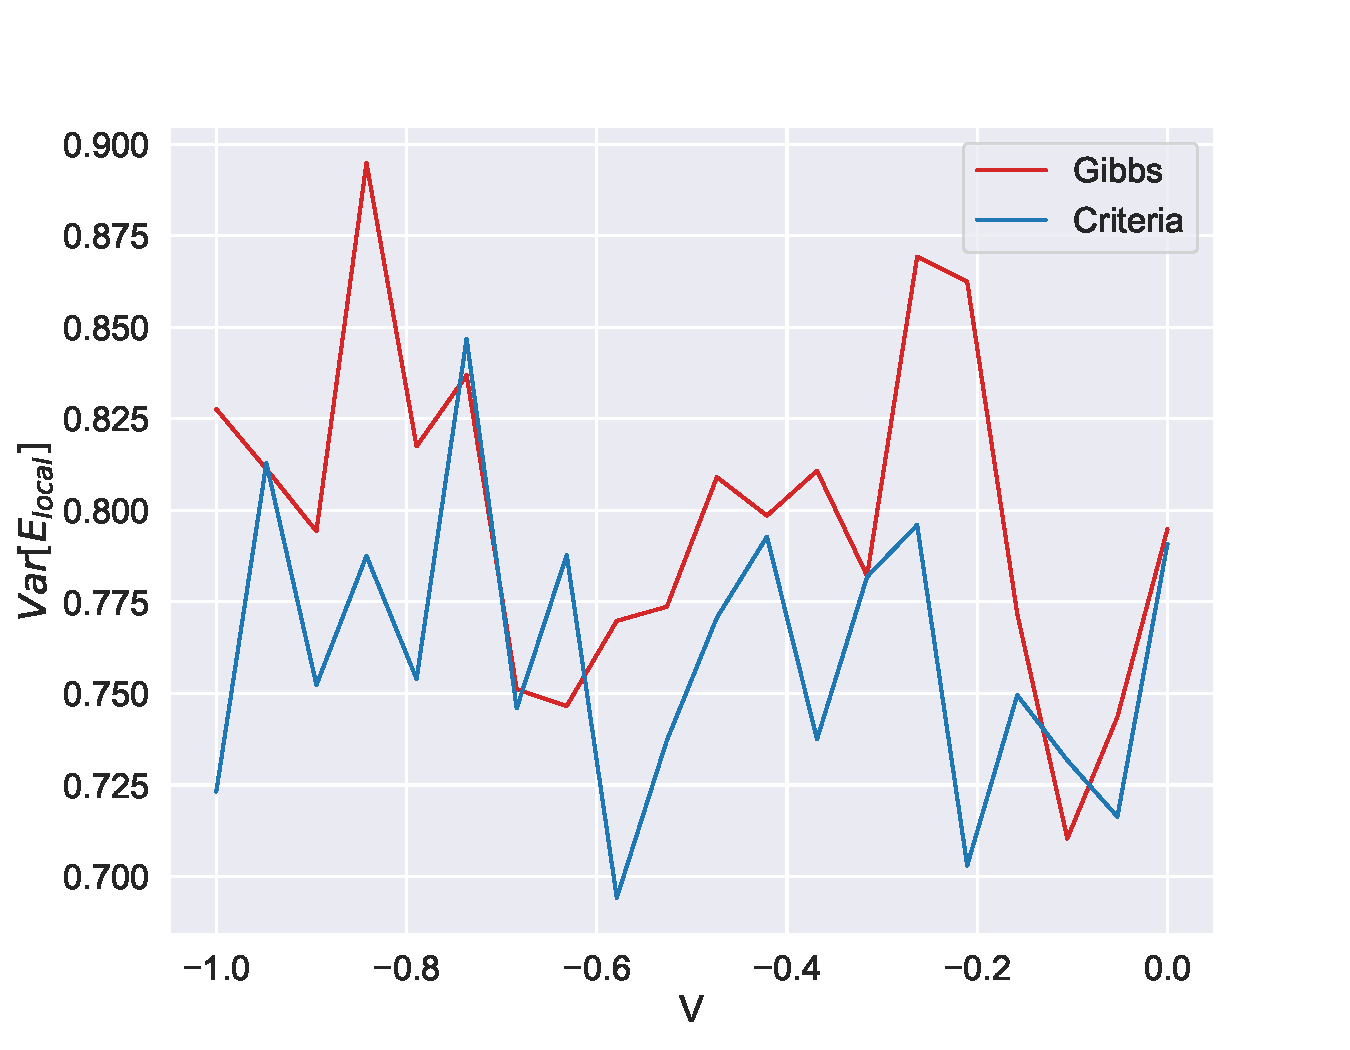
\includegraphics[width=0.95\textwidth]{Figures/Plots/met_gibbs_V.pdf}
  \end{center}
  \caption{The variance of two RBMs where one uses the Gibbs sampling method, and the other uses a conditional acceptance criteria of the RBM's internal energy, here with $\mgC$ Monte Carlo cycles. The quantum system is the Lipkin model with $16$ particles and $\varepsilon = \mgeps$ and $W = \mgW$.}
\end{figure}

We see that Metropolis-Hastings with acceptance criteria in general has a lower variance than Gibbs sampling. Here we have only used $k = 2$ Gibbs cycles, sampling back and forth between the visual and hidden layer, which may contribute somewhat to higher variance. Still, the difference here does not weigh up for the computation time difference. The efficiency increase is largely based on hardware, so we will here not compare the two, but even with simple parallelization the variance difference above could be made up for by an increase in samples instead.



